\chapter{Topology Control}
\label{math0}

\begin{flushright}
\textit{``If it's just turning the crank it's algebra, but if it's got an idea in it, it's topology.''}\\
-- Solomon Lefschetz
\end{flushright}

Topology began with the study of curves, surfaces and other objects in the plane and 3D space.
One of the central ideas in topology is that spatial objects like circles and spheres can be treated as objects in their own right, and knowledge of objects is independent of how they are embedded in space.
Topology can be used to abstract the inherent connectivity of objects while ignoring their detailed form.\\
For example, the figures shown in picture \ref{fig:topology_examples} illustrate the connectivity of a number of topologically distinct surfaces and at the same time links them to a common denominator -- solid parallel edges join one another with the orientation indicated by arrows, dashed lines show edges that remain free \citep[][cf. p.1]{Weisstein2012}:
%Figure
\begin{figure}[ht]
\centering
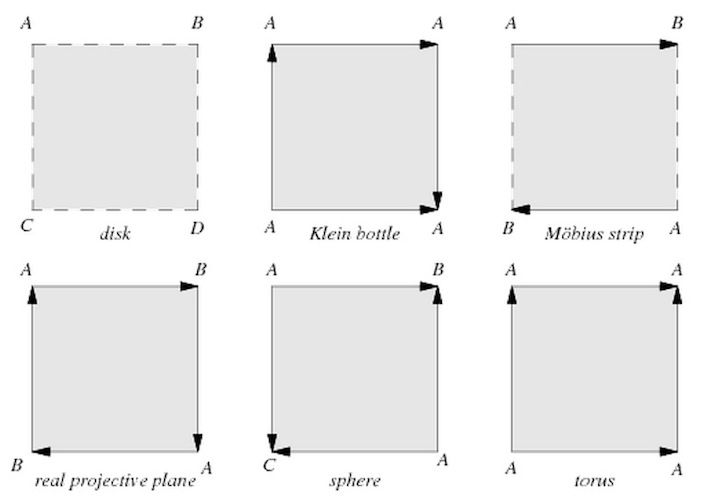
\includegraphics[width=0.6\textwidth]{topology_examples.jpg}
\caption{Connectivities of prominent 2D manifolds.}
\label{fig:topology_examples}
\end{figure}\\
Although topology is a comparatively young field in the history of mathematics, it would be futile trying to give a comprehensive explanation of the entire field\footnote{ The beginnings of Topology are closely related to advances in set theory at the end of the $19^{th}$ century. An iconic date for the commencement is the formal definition of metric spaces by \textit{Maurice Fréchet} in 1906. Today topology can be divided into algebraic topology (which includes combinatorial topology), differential topology, geometric topology and low-dimensional topology known as point-set topology \citep[][cf. p.2]{Weisstein2012}.}.\\
For our purposes we split this chapter in two parts, firstly we introduce the most important definitions in section \ref{math1}.
Many of the presented concepts will be already known, at least in an intuitive way, but in order to proceed to more demanding theories, it is necessary to formulate them in an concise and unifying manner.
Key ingredient is the notion of 'Simplicial Complexes' in \ref{math_simplicalcomplexes}, a powerful abstraction for spaces with triangulations, subsequently constructed by gluing together series of lower-dimensional simplices.\\
The second chapter \ref{math2} then will introduce a set of mathematical tools to describe and compute geometric features like handles and tunnels in a precise and rigid way.
As a means to do this, it will be necessary to introduce advanced theories like 'Filtration' and 'Topological Persistence', first described by Edelsbrunner \citep[cf.][]{Edelsbrunner2000}.
Some of the definitions might seem overly abstract at times, but as it turns out, describing and finding handles or tunnels in a mathematically sound manner is a challenging task.

What we ultimately want to achieve, by mobilizing all the mathematical machinery, is best expressed by the relation expressed in equation \ref{mother_equation}:
\begin{equation}
	\underbrace{ \chi = \sum (-1)^{n} \, \beta^{n}}_{Euler-Poincaré}
	\hspace{3ex} \longrightarrow \hspace{1ex}
	\underbrace{ \beta^{n}}_{n-Betti} =
	\underbrace{ rank ~{Z}^{n} - rank ~\mathrm{B}^{n}}_{Homology~groups} =
	\underbrace{ |\Prefix^{+}{\sigma^{n}}|-|\Prefix^{-}{\sigma^{n+1}}|}_{Filtration}
\end{equation}\\
In a nutshell what it says, is that the topological important information is connected to the filtration of simplices.
The Euler-Poincaré characteristic representing the topological important information can be calculate with Betti numbers.
This conclusion can be further used because the Betti numbers in turn, represent ranks of homology.
In other words, at the end we want to find groups of chains and circles that are either trivial or bounding.
All of that and more will be covered in this chapter.
%Figure
%\begin{figure}[ht]
%\centering
%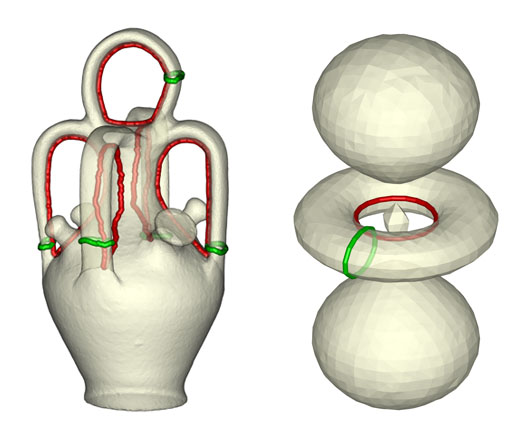
\includegraphics[width=0.1\textwidth]{loops_handles.jpg}
%\caption{Tunnel (red) and handle (green) loops \citep[cf.][]{Dey2012}.}
%\label{fig:loops_handles}
%\end{figure}\\

Note that the following expositions are somewhat informal in so far that they focus on conveying the concepts rather than building a strict series of deductions.
Lemmata or proofs will only be given if they are of importance for the understanding, further details and side-notes generally refer to sections in the appendix.

\newpage
\section{Mathematical Primer}
\label{math1}

Before we introduce any concepts it is important to stress that the field of topology is of axiomatic nature.
Therefore it can appear that already known structures are convoluted by cryptic terminology, but as often with axiomatic fields we have to accept these definitions as new.
For example, we mostly imply metric spaces when talking about ``a space'', when the differences are actually quite profound, see figure \ref{fig:spaces}:
%Figure
\begin{figure}[ht]
\centering
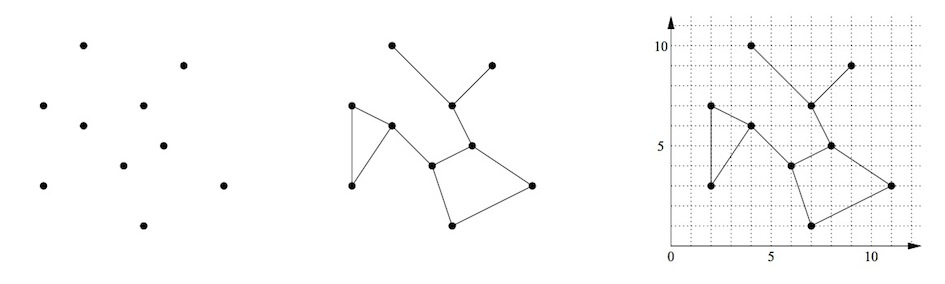
\includegraphics[width=0.95\textwidth]{spaces.jpg}
\caption{A point-, topological- and metric-space.}
\label{fig:spaces}
\end{figure}\\
A space can be a set of points without any structure.
For a topological space we need knowledge of the connectivity of the space, each point \textit{knows} which points are near it, that is its neighborhood.
To form a metric space we additionally need an associated metric, which enables us to measure distances and in turn, implicitly
defines neighborhoods.
Consequently any metric space is a topological one.
This means the geometry and topology of a space are fundamentally related, as they are both properties of a certain space.
However, the questions we are interested in are often topological in nature, and we may solve them easier by focusing on the topology and not on its geometry.
To do so, we need to identify intrinsic properties of spaces, especially the ones that are not changing -- so called invariants of the space\footnote{ This definition, to classifying geometries by their underlying symmetry groups, was coined by \textit{Felix Klein} (1849-1925) under the name ``Erlanger Programm''.
\begin{quote} \textit{``... Euclidean metric geometry can be described as the study of properties unchanged be the group of all rigid motions. ... All of these characteristics are dependent on two fundamental invariants in terms of which that can be expressed, namely, distance and angle. Euclid's pure geometry of measurement assumed that the effects of motion must leave size invariant. The issue of whether this is a good assumption for motion in the real world arises in twentieth-century physics.''} \citep[p.405]{Kramer1982} \end{quote}
} \citep[][cf. pp.1-5]{Zomorodian1996}.

\subsection{Topology}
\label{math_topology}

A topology is simply a system of sets that describe the connectivity of a set.
Formally a topology on a set $\mathrm{X}$ is a subset $\mathrm{T} \subseteq 2^{X}$ such that\footnote{ Definitions and figures in this chapter stem from mainly three resources and won't be cited individually:\begin{itemize}
\item \citep[][]{Hatcher2002} is a freely available textbook on algebraic topology and very often cited.
\item \citep[][]{Zomorodian1996} the PhD thesis of Prof. Afra Zomorodian, which features an extensive introductory chapter on topology (often citing Hatcher).
\item \citep[][]{Weisstein2002} the online resources of MathWorld, written and curated by \textit{Eric W. Weisstein}, hosted/sponsored by and licensed to 'Wolfram Research, Inc'.\end{itemize}}:
\begin{enumerate} \setlength{\itemsep}{0cm} \setlength{\parskip}{0cm}
	\Item $\text{If } \mathrm{A_{1}}, \mathrm{A_{2}} \in \mathrm{T} \text{, then } \mathrm{A_{1}} \cap \mathrm{A_{2}} \in \mathrm{T}.$
	\Item $\text{If } \{\mathrm{A_{j}} | j \in J\} \subseteq \mathrm{T} \text{, then } \cup_{J} \mathrm{A_{j}} \in \mathrm{T}.$
	\Item $\emptyset, \mathrm{X} \in \mathrm{T}.$
\end{enumerate}
We endow a set with structure to get the pair $\mathbb{X} = (\mathrm{X},\mathrm{T})$, called a topological space with any $\mathrm{A}_{i} \in \mathrm{T}$ an open set and its complements in $\mathrm{X}$ closed.
A continuous function between two topological spaces $f: \mathbb{X}_{1} \rightarrow \mathbb{X}_{2}$, is called a map if for every open set $\mathrm{B} \in \mathbb{X}_{2}$, $f^{-1}(\mathrm{B})$ is also open in $\mathbb{X}_{1}$, i.e. for every object in $\mathbb{X}_{2}$ exists an unique object in $\mathbb{X}_{1}$.\\
A homeomorphism $f: \mathbb{X}_{1} \rightarrow \mathbb{X}_{2}$ is a 1-1 onto function such that both $f$ and $f^{-1}$ are continuous, i.e. they have the same topological type $\mathbb{X}_{1} \approx \mathbb{X}_{2}$.
Homeomorphisms partition the class of topological spaces into equivalence classes and a fundamental problem in topology is characterizing these classes of homeomorphic spaces.

\subsection{Manifolds}
\label{math_manifolds}

A topological space may be viewed as an abstraction of a metric space.
Similarly, manifolds generalize the connectivity of $n$-dimensional Euclidean spaces $\mathbb{R}^{n}$ by being locally similar, but globally different, thus allowing to describe more complicated structures in terms of well-understood properties of Euclidean space.
A homeomorphism mapping the local ``area'' $\mathrm{U} \subseteq \mathbb{X}$ to an open subset of $\mathbb{R}^{n}$ is called a chart: $\varphi : \mathrm{U} \rightarrow \mathbb{R}^{n}$.
Formally a manifold is a topological space with a chart defined for every $x \in \mathbb{X}$.\\
For example, all neighborhoods on the 2-sphere $\mathcal{S}^{2}$ are homeomorphic to open disks.
Likewise the circle or 1-sphere $\mathcal{S}^{1}$ is a 1-manifold as every point has a neighborhood homeomorphic to an open interval in $\mathbb{R}^{1}$.
It is also the only compact 1-dimensional manifold.
Manifolds are generally the only topological spaces we are interested in.
%Figure
\begin{figure}[ht]
\centering
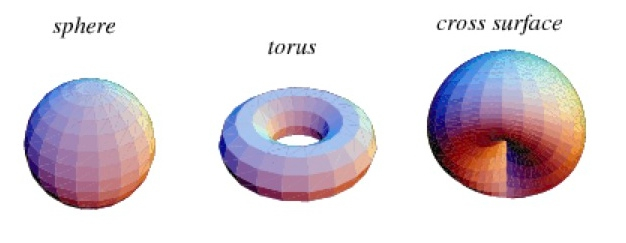
\includegraphics[width=0.60\textwidth]{manifolds.jpg}
\caption{Complete homeomorphism list for compact, boundaryless 2-dim. manifolds.}
\label{fig:manifolds}
\end{figure}\\
Another important attribute is compactness: A compact manifold can be embedded in $\mathbb{R}^{n}$ if it has finite extent, i.e. it can be covered by finitely many charts $\varphi_{n}$ -- thus all compact surfaces are triangulable \citep[which was first shown by][]{Rado1925}.
Compact manifolds in two dimensions are completely classified by two further attributes, namely orientation and genus, see picture \ref{fig:manifolds} and table \ref{tab:manifolds}:
\begin{table}[hbt]
\medskip
\setlength{\tabcolsep}{15pt}
\renewcommand{\arraystretch}{1.0}
   \centering
\begin{tabular}{ l || c | c | c } \centering
	\textbf{genus}		& 0			& 1				& 2 \\ \hline \hline
	\textbf{orientabel}	& sphere		& torus 			& double torus \\ \hline
	\textbf{nonorientable}	& -			& cross-cap		& Klein bottle \\
\end{tabular}
   \medskip
   \caption{Classes of 2-dimensional compact manifolds with low genus.}
   \label{tab:manifolds}
\end{table}\\
The genus is maybe the best known invariant property, as it intuitively describes the number of holes in a surface and we will see its connection to the more general notion of the Euler characteristic\footnote{ In higher-dimensional manifolds, the Euler characteristic is replaced by the concept of Betti numbers and homology/cohomology, as it gives rise to a broader framework of invariants, called functors. For definitions of homology and Betti numbers, see section \ref{math_homology}, respectively the glossary in appendix \ref{appendix_glossary}.} later in section \ref{math_euler}.
The genus can also be seen as the maximum number of cuttings along non-intersecting closed simple curves that can be drawn on the surface without disconnect the manifold into two.\\
The second invariant, orientability, describes whether it is possible to give all local charts $\varphi_{n}$ an ordering of either right- or left-handedness, without any two neighboring charts disagreeing globally.
Formally we will define this concept in the next section \ref{math_simplicalcomplexes}.\\
Using the connected sum, the homeomorphism problem is fully resolved for 2-manifolds\footnote{ \textit{Grigori Perelman} showed that 3-manifolds can also be decomposed into pieces with uniform geometry, whereas the problem is proven to be undecidable for higher dimensions \citep[][]{Morgan2007}.}, as every compact surface is homeomorphic to a sphere, the connected sum of tori, or the connected sum of cross surfaces\footnote{ Hence for any closed 2-manifold embedded in 3-dimensional space that can not be oriented, it follows, that it must have at least one self-intersection and any orientable 2-manifold without boundary is homeomorphic to a sphere with $n$-handles, i.e. its genus.}!

\subsection{Simplical Complexes}
\label{math_simplicalcomplexes}

At the beginning of the chapter in picture \ref{fig:topology_examples} we have seen that a torus, like a projective plane\footnote{ A sphere with one cross-cap has traditionally been called a real projective plane. The cross-cap is one of the three possible surfaces obtained by sewing a Möbius strip to the edge of a disk -- the other two are the Boy surface and Roman surface, see picture \ref{fig:nonorientable_surfaces}. A sphere with two cross-caps having coinciding boundaries is topologically equivalent to a Klein bottle.} and a sphere, all can be obtained from a
square by identifying the edges with certain directions and gluing them together accordingly.
Cutting a square trivially along a diagonal produces two triangles that can be easily further subdivided, so each of these surfaces in turn can be reduced to triangles.
Together with the result from the last section \ref{math_manifolds}, that all compact 2-manifolds can be assembled by combining spheres, tori and cross-caps, we have proven that in fact all closed surfaces can be constructed from triangles.\\
Thus we have a single building block to construct a large class of 2-dimensional spaces and the idea now is to generalize this for any dimension:
The $n$-dimensional analog of the triangle is the convex hull of $n$+1 affinely independent points $\mathcal{V} = \{v_{0}, v_{1}, \dots , v_{n}\}$, it is called the $n$-simplex: $\sigma^{n}_{i}$, with $n$ and $i$ denoting the dimension and index: $i,n \in \mathbb{N}$.
Simplices have familiar names for low dimensions, see figure \ref{fig:n-simplices}:
%Figure
\begin{figure}[ht]
\centering
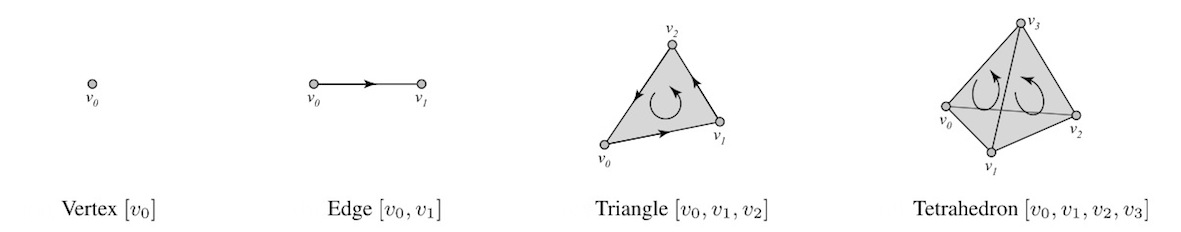
\includegraphics[width=1.0\textwidth]{n-simplices.jpg}
\caption{Oriented $n$-simplices, $0 \leq n \leq 3$.}
\label{fig:n-simplices}
\end{figure}\\
Now a simplicial complex $\mathrm{K}$, is a finite set of simplices such that every subset $\mathrm{T} \subseteq \mathcal{V}$ is also in $\mathrm{K}$, and the nonempty intersection of any two simplices, again is a subset in $\mathrm{K}$.
The dimension $n$ of $\mathrm{K}^{n}$ is defined as the maximum dimension of its simplices: $max_{n}\{\sigma^{n}_{i}\}$.\\
That is to say, that a simplicial Complex is a set of elements, i.e. simplices of different dimension, that built up and represent a manifold.
The cumbersome definition stems from the fact that we want to exclude certain ill-formed sets, shown in figure \ref{fig:simplical_complexes}.\\
To put this into context, a triangulation of a topological space $\mathbb{X}$ is a simplicial complex $\mathrm{K}$.
Formally this is the case if the underlying space of the simplicial complex is isomorphic to the topological space: $||\mathrm{K}|| \approx \mathbb{X}$.
Thus, two simplicial complexes $\mathrm{K}$ and $\mathrm{L}$ are isomorphic if and only if their topological spaces are: $\mathbb{X}_{\mathrm{K}} \approx \mathbb{X}_{\mathrm{L}}$.
%Figure
\begin{figure}[ht]
\centering
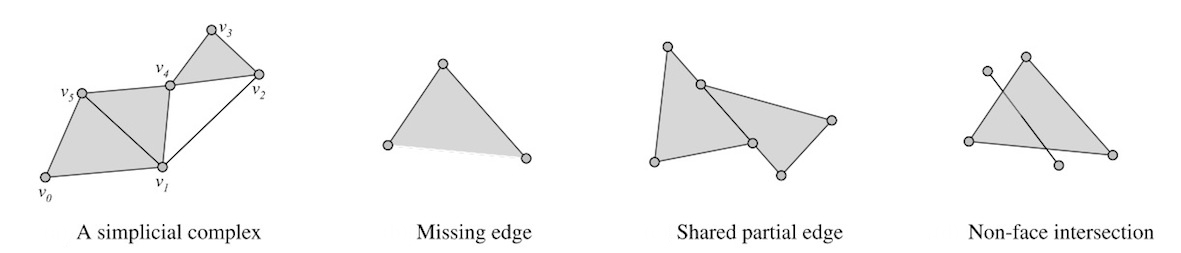
\includegraphics[width=1.00\textwidth]{simplical_complexes.jpg}
\caption{One simplicial complex and three unions that are not complexes.}
\label{fig:simplical_complexes}
\end{figure}\\
For purposes of homology it is important to keep track of the order of the simplices, so $n$-simplex really means $n$-simplex with ordering, which as a by-product, determines orientation:
Two $n$-simplices sharing a ($n$-1)-simplex are consistently oriented if they induce different orientations.
A triangulable $n$-manifold is orientable if all simplices can be oriented consistently, otherwise it is nonorientable, see figure \ref{fig:nonorientable_surfaces}.
Orientations are normally graphically indicated by using arrows, as shown in figure \ref{fig:example_orientation}.
Note that in three dimensions, there is no unbounded non-orientable surface which does not intersect itself\,\footnote{ See appendix \ref{appendix7}, for a very elegant proof of this statement.}.
%Figure 
\begin{floatingfigure}[r]{0.30\textwidth}
\centering
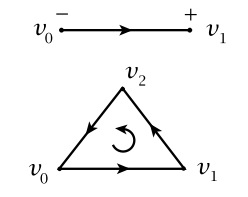
\includegraphics[width=0.25\textwidth]{example_orientation.jpg}
\caption{Orientation.}
\label{fig:example_orientation}
\end{floatingfigure}
We can generalize the idea now for any dimension $n \geq 1$:
Then an orientation of a $n$-simplex $\sigma^{n}$, is an equivalence class of orderings, written $[\sigma]$, of its vertices: $\sigma = \{v_{0}, v_{1}, \dots , v_{n}\}$, where: $(v_{0}, v_{1}, \dots , v_{n}) \sim (v_{\tau(0)}, v_{\tau(1)}, \dots , v_{\tau(n)})$, are equivalent orderings if the parity of the permutation $\tau$ is even\footnote{ For any finite set $\mathrm{X}$ with an ordering and at least two elements, the bijective mapping $\tau : \mathrm{X} \rightarrow \mathrm{X}$, falls into two classes of equal size, i.e. the even and odd permutations. The parity a permutation is then defined as the number of inversions for $\mathrm{N}(\tau)$, of pairs of elements $x_{i}, x_{j} \in X$, such that $x_{i} < x_{j}$ but $\tau(x_{i}) > \tau(x_{j})$, intuitively this denotes the number of occurred swaps.}.\\
It is worth noting that simplicial complexes, by definition, are combinatorial objects with topology and don't necessarily have to utilize geometry.
If the topology gets separated, $\mathrm{K}^{*}$ is called an abstract simplicial complex\footnote{ Actually written down for simplicial complexes, the mathematical definition of this vertex scheme, strikingly resembles the connectivity list of an \textit{.obj}, \textit{.ply} or \textit{.off} file.}.
%Figure
\begin{figure}[ht]
\centering
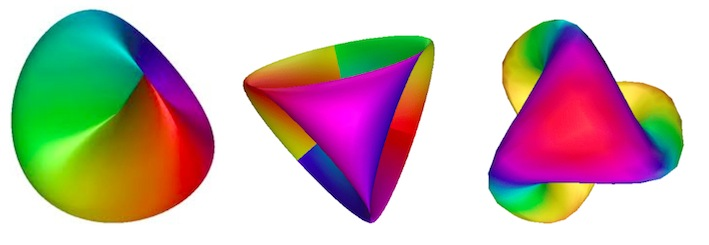
\includegraphics[width=0.45\textwidth]{nonorientable_surfaces.jpg}
\caption[Non-orientable surfaces]{Basic non-orientable surfaces: Cross-cap, Roman and Boy surface.}
\label{fig:nonorientable_surfaces}
\end{figure}

\subsection{General Euler Characteristic}
\label{math_euler}

Next to orientability the genus is the second most well known invariant for classifying $2-$manifolds.
We already have a intuitive notion for it, as it represents the number of holes\footnote{ Though even for non pathological cases it can be very hard to ``see'' the genus of a given surface. A famous example is the so called ``House with two rooms'', illustrated in appendix \ref{two_rooms}.}, but with simplicial complies at our disposal we can formulate this concept in a generalized and formal adequate way for any $n$-manifold.\\
The Euler characteristic is defined for a simplicial complex $\mathrm{K}$ with $|\sigma^{n}|$ finitely many $n$-simplex as the number of even- minus the number of odd-dimensional simplices:
\begin{equation} \label{eq:euler_characteristic}
\chi(\mathrm{K}) = \sum_{n = 0}^{dim \mathrm{K}} (-1)^{n} |\sigma^{n}|
\end{equation}
Which in the $2$-dimensional case leads to the well known relation:
\begin{equation*}
\chi(\mathbb{M}_{2}) = |\sigma^{0}| - |\sigma^{1}| + |\sigma^{2}| = vertices - edges + faces
\end{equation*}
And we get for the tetrahedron $\sigma^{3}$ in picture \ref{fig:simplical_complexes}: $\chi(\sigma^{3}) = 4 - 6 + 4 = 2$, which by definition is a triangulation of the sphere $\mathcal{S}^{2}$, thus defining the homeomorphism for any convex polyhedron $\mathbb{M}$ as $\chi(\mathbb{M}) = 2$, respectively $\chi(\mathbb{M}) \simeq \chi(\mathcal{S}^{2})$.\\
The Euler characteristic of a $\mathrm{K}$ depends only on its homotopy type, no matter how it is geometrically represented, i.e.
it is an integer invariant for $|\mathrm{K}|$, the underlying space.
We already know that any compact orientable surface is homeomorphic to a sphere or $n$ connected tori.
Thereby we can give an atomic formula for any connected sums of orientable $\mathbb{M}_{sum}$ or nonorientable $\mathbb{N}_{sum}$ manifolds\footnote{ An informal explanation for the added $(-2g)$ and $(-g)$ terms is, that, to connect the surfaces one either has to cut out a disk on either tori $(-2)$, or cut two disks and insert a projective plane $(-2+1)$, g-times.}: 
\begin{equation}
\chi(\mathbb{M}_{sum}) = 2 - 2g \text{, respectively: } \chi(\mathbb{N}_{sum}) = 2 - g
\end{equation}
%Figure
\vspace*{-4ex}
\begin{figure}[ht]
\centering
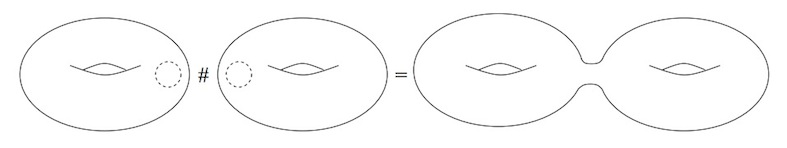
\includegraphics[width=0.8\textwidth]{connected_sum.jpg}
\caption{A double torus, as the connected sum of two tori.}
\label{fig:connected_sum}
\end{figure}

\subsection{Homotopy}
\label{math_homotopy}

Two continuous functions from one topological space to another are called homotopic, if one can be continuously deformed into the other.
The deformation then is called the homotopy between the two functions and an equivalence relation on topological spaces\footnote{ Equivalence classes under $\simeq$ are called homotopy types. Like any equivalence relation they partition a set so that every element of the set is a member of one and only one cell of the partition. The intersection of any two different cells must be empty and the union of all the cells equals the original set. They are reflexive: $\mathrm{X} \simeq \mathrm{X}$, symmetric: $\mathrm{X} \simeq \mathrm{Y} \, \Rightarrow \, \mathrm{Y} \simeq \mathrm{X}$ and transitive: $\mathrm{X} \simeq \mathrm{Y} \, \& \, \mathrm{Y} \simeq \mathrm{Z} \Rightarrow \mathrm{X} \simeq \mathrm{Z}$.}.
More precisely, two continuous maps $f, g: \mathbb{X}_{1} \rightarrow \mathbb{X}_{2}$ are homotopic, if a continuous function exists $\mathrm{F}: \mathbb{X}_{1} \times [0,1] \rightarrow \mathbb{X}_{2}$, so that:
\begin{equation}
	\mathrm{F}(x, 0) = f(x) \text{ and } \mathrm{F}(x, 1) = g(x) \text{, for all } x \in \mathbb{X}_{1}
\end{equation}
To give an example: Any two continuous real functions $f, g: \mathbb{R} \rightarrow \mathbb{R}$ are trivially homotopic via $\mathrm{F}(x,t) = (1-t) \cdot f(x) + t \cdot g(g)$.
If $f$ is homotopic to a constant map, i.e. $f \simeq const.$, then $f$ is called nullhomotopic.
As with functions, two spaces $\mathbb{X}_{1}$ and $\mathbb{X}_{2}$ are homotopy equivalent if they can be transformed into one and another by continuous bending, shrinking and expanding operations, see picture \ref{fig:homotopy}.
%Figure
\begin{figure}[htb]
\centering
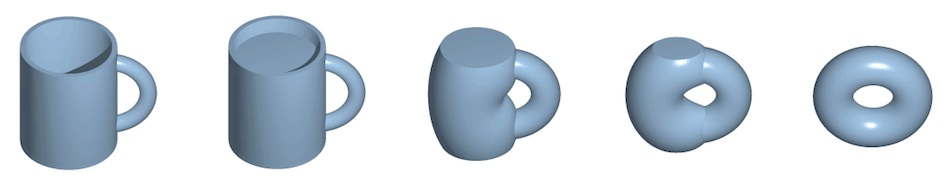
\includegraphics[width=0.9\textwidth]{homotopy.jpg}
\caption{A famous example for homotopic equivalence are a coffee cup and a torus.}
\label{fig:homotopy}
\end{figure}\\
A topological space $\mathbb{X}$ is said to be contractible or nullhomotopic if $\mathbb{X}$ is homotopy equivalent to a point, i.e. $\mathbb{X} \simeq \sigma^{0}$.\\
It is important not to mix up homeomorphism with homotopy.
For example, a cylinder is not homeomorphic to a circle, but homotopy equivalent to it, as it may continuously be shrunken via a deformation retraction\footnote{ Deformation retraction is a special case of a homotopy, with the requirement that the target space is a subspace. The retraction of a space $\mathbb{X}$ onto a subspace $\mathrm{A}$ is a family of continuous maps $f_{t}: \mathbb{X} \rightarrow \mathrm{A}, t \in [0,1]$, so that $f_{0}$ is the identity map: $f_{0}(\mathbb{X}) = \mathbb{X}$, and $f_{1}(\mathbb{X}) = \mathrm{A}$. In other words, starting from the original space $\mathbb{X}$ at time $0$, we continuously deform the space until it becomes the subspace $\mathrm{A}$ at time $1$. This is done without ever moving the subspace $\mathrm{A}$ in the process.}.
Thus, two spaces with a different topological type can still have the same homotopy type, but all homeomorphic spaces are homotopic: $\mathbb{X}_{1} \approx \mathbb{X}_{2} \, \Rightarrow \, \mathbb{X}_{1} \simeq \mathbb{X}_{2}$ but not the other way around.

\subsection{The Fundamental Group}
\label{math_fundamental_group}

We saw in the last section that two maps are homotopic if one can be continuously deformed into the other.
Now this idea gets applied to maps on surfaces, called paths.
Paths that begin and start at the same basepoint $x_{bp}$, namely loops, are of special concern and used to characterize the so called fundamental group.\\
Loops that are boundaries of a disk are contractible and belong to the same class as the trivial loop, which never leaves its basepoint.
If we find non-bounding loops, they form a different class, see picture \ref{fig:fundamental_group_torus}.
%Figure
\begin{figure}[htb]
\centering
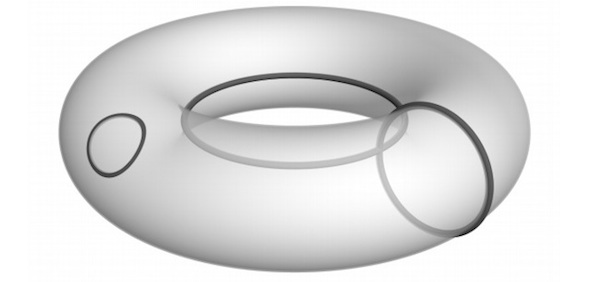
\includegraphics[width=0.45\textwidth]{fundamental_group.jpg}
\caption{One boundary loop (on the left) and two non-bounding loops on a torus.}
\label{fig:fundamental_group_torus}
\end{figure}
\begin{equation}
	f_{loop}: [0,1] \rightarrow \mathbb{X} ~~ \text{ with }~~ f_{loop}(0) = x_{bp} = f_{loop}(1)
\end{equation}
The non-bounding loops define the fundamental group.
Formally the fundamental group of a topological space is the group formed by the set of equivalence classes of all loops with the same initial and final basepoint, under the equivalence relation of homotopy:
\begin{equation}
	\pi(\mathbb{X}, x_{bp}) = \{ f_{loop}: [0,1] \rightarrow \mathbb{X} ~|~ f_{loop}(0) = x_{bp} = f_{loop}(1)\}_{h}
\end{equation}
For a non-pathological spaces, i.e. path-connected spaces, the basepoint is irrelevant and we refer to the group as $\pi_{1}(\mathbb{X})$.
For example, any loop drawn on the sphere is bounding, so $\pi_{1}(\mathcal{S}^{2}) \cong \{0\}$ where $\cong$ denotes group isomorphism\footnote{ Admittedly, it is hard not to get confused by all the introduced -morphisms (left alone, that there are even more esoteric ones). Isomorphism is a bijective group homomorphism, which in turn must not be confused with homeomorphism. Contrary to homeomorphism, homomorphism is structure-preserving.} and $\{0\}$ is the trivial group.\\
Each homotopy class consists of all loops which wind around the circle a given number of times.
So the fundamental group of the circle is isomorphic to the additive group of integers $\mathbb{Z}$.
Intuitively then, $\pi_{1}(\mathcal{S}^{1}) = \mathbb{Z}$ and similarly the two non-bounding loops in picture \label{fig:fundamental_group} generate the fundamental group of a torus: $\pi_{1}(\text{Torus}) \cong \mathbb{Z} \times \mathbb{Z}$.\\
The fundamental group, in fact, measures the 1-dimensional hole structure of a space.
Following is table \ref{tab:fundamental_group} of the fundamental group for some common spaces:
\begin{table}[htpb]
\medskip
\setlength{\tabcolsep}{25pt}
\renewcommand{\arraystretch}{1.25}
   \centering
\begin{tabular}{ l | c | c } \centering
	\textbf{Space}	& \textbf{Symbol}				& \textbf{$\pi_{1}$} \\ \hline \hline
	Circle			& $\mathcal{S}^{1}$			& $\mathbb{Z}$ \\
	Torus			& $\mathcal{T}^{2}$			& $\mathbb{Z}^{2}$ \\
	Projective plane	& $\mathbb{R}\mathrm{P}^{2}$	& $\mathbb{Z}$ \\
	Sphere			& $\mathcal{S}^{2}$			& $0$ \\
\end{tabular}
	\bigskip
	\caption{Fundamental group for various spaces.}
	\label{tab:fundamental_group}
\end{table}\\
The fundamental group is one in a series of homotopy groups $\pi_{n}(\mathbb{X})$ that study higher dimensional holes.
The homotopy groups $n > 1$ extend the notion of a loop to $n$-dimensional circles and capture the homotopy
classes of these circles.

\subsection{Chains and Circles}
\label{math_chainloops}

As before, we can now generalize the concept of paths and loops with the help of simplicial complexes and use it to define another topological invariant, homology.\\
A path $c$ constructed with simplices of dimension $n$ is called a $n$-chain of the simplicial complex $\mathrm{K}$.
With $\sigma_{i}^{n} \in \mathrm{K}, ~k_{i} \in \mathbb{Z}$ and the brackets $[\cdot]$ indicating orientation as introduced in section \ref{math_simplicalcomplexes}, we define a $n$-chain as the sum of $i$ connected simplices:
\begin{equation}
	\mathrm{c}^{n} = \sum_{i} k_{i} [\sigma_{i}^{n}] ~\text{ respectively the chain group of all $n$-chains: } \mathrm{C}^{n} = \{ \cup_{\mathrm{K}} ~ \mathrm{c}^{n} \}
\end{equation}
We also define a commutative addition for chains with integer coefficients modulo 2.
In other words, the sum of two $n$-chains $c$ and $d$ is the symmetric difference of the two sets: $c+d = (c \cup d) - (c \cap d)$, preventing multiple instances of an element $\sigma^{n}$ in the set.\\
The chain group $\mathrm{C}^{n}$ is the set\footnote{ To be precise, this set forms a free Abelian group on the oriented $n$-simplices: $\langle \mathrm{C}^{n}, + \rangle$. Which means, they form a basis and the entirety of the elements can be written as linear combinations of the basis.\\ Abelian groups are structures of abstract algebra, studied in group theory. As we are interested in characterizing the topology of spaces, group theory is a related classification systems that yields many interconnections. Although promising powerful tools to define equivalence relations, the exploration of this relation is beyond the scope of this thesis and my knowledge thereof \citep[for an in depth introduction to the field of geometric group theory, see][]{Stillwell1993}.} of all chains with dimension $n$, hence $\mathrm{K}$ has a chain group in every dimension.
These chain groups $\mathrm{C}^{n}$ are structurally related in the way that $(n\text{-1})$-chains form the boundaries of $n$-chains, i.e. every tetrahedron $\sigma^{3}$ is bounded by four triangles $\sigma^{2}_{\{1-4\}}$ and every triangle $\sigma^{2}$ is bounded by three edges $\sigma_{\{1-3\}}^{1}$ and so forth.
We now define this relation formally via the boundary operator:
\begin{equation} \label{eq:boundary}
	\partial \,\sigma^{n} = \partial \,\{ v_{0}, \dots , v_{n} \} = \sum_{i}^{n} \,\{v_{0}, \dots, \hat{v}_{i}, \dots, v_{n}\}
\end{equation}
where $\hat{v}_{i}$ is the simplex that gets deleted from the sequence.
We extend this operator to entire chain groups, $\partial_{n}: \mathrm{C}^{n} \rightarrow \mathrm{C}^{n-1}$ and interpret $\partial_{0} \equiv \emptyset$.
The entire series of the groups that are connected via the boundary operator is then called a chain complex $\mathrm{C}^{\mathrm{K}}$ : $\mathrm{C}^{\mathrm{K}} = \mathrm{C}^{n} \overset{\partial_{n}}{\longrightarrow} \mathrm{C}^{n-1} \overset{\partial_{n-1}}{\longrightarrow} \dots \overset{\partial_{1}}{\longrightarrow} \mathrm{C}^{0} \overset{\partial_{0}}{\longrightarrow} \emptyset$\\
This gives us the definition of a $n$-circles as $n$-chains that have no boundary.
As an example consider the triangle in figure \ref{fig:example_orientation}, with the obvious $1$-circle, formed by its edges: $\partial_{2} \sigma^{2} = \partial_{2} \{ \sigma^{1}_{0}, \sigma^{1}_{1}, \sigma^{1}_{2} \} = \{v_{1}, v_{2}\} + \{v_{0}, v_{2}\} + \{v_{0}, v_{1}\}$, now taking the boundary of the boundary we can see: $\partial_{1} (\{v_{1}, v_{2}\} + \{v_{0}, v_{2}\} + \{v_{0}, v_{1}\}) = 2v_{2}+2v_{1}+2v_{0}$ and with the addition defined modulo 2, the results is: $2v_{2}+2v_{1}+2v_{0} = \emptyset$.
This is intuitively correct, as the boundary of a triangle is a cycle, and a cycle does not have a boundary.
In fact, this intuition generalizes to chain groups of any dimension\footnote{ We omit the proof, but it is rather straight forward, as $\partial_{n} \partial_{n-1} = \sum \sum [\dots]$ mod2 always cancels out.}: $\partial_{n}(\partial_{n-1}) = \emptyset$.
In other words, the $n$-cycles are the kernel\footnote{ The boundary operator $\partial_{n}$ is a group homomorphism, hence the kernel is defined as the set of all elements which are mapped to the identity element of $\partial_{n-1}$. The image, analogous to real functions, is the range of all mapped elements, i.e. all chains for which $\partial_{n+1}$ is defined.} of $\partial_{n}$ and thereby form a subgroup of the chain group $\mathrm{C}^{n}$, which is called the cycle group: $\mathrm{Z}_{n} = ker ~ \partial_{n} = \{ c \in \mathrm{C}^{n} ~ | ~ \partial_{n} \, c = 0\}$.\\
If we recall the three circles on the torus shown in figure \ref{fig:fundamental_group_torus}, we see that apart from the boundary loops, there are also non-bounding loops.
The entirety of loops can be defined by the image of all ($n$+1)-boundaries: $\mathrm{B}_{n} = im ~ \partial_{n+1} = \{ c \in \mathrm{C}^{n} ~|~ \exists d \in \mathrm{C}^{n+1} : c = \partial_{n+1}(d) \}$.
%Figure
\begin{figure}[htb]
\centering
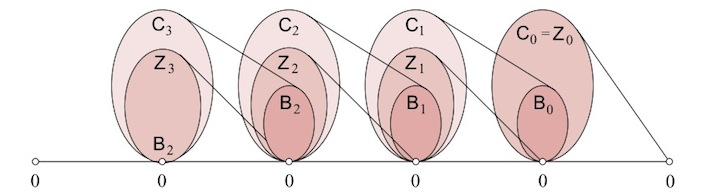
\includegraphics[width=0.70\textwidth]{chain_complex.jpg}
\caption{The chain complex for a $3$-dimensional simplicial complex.}
\label{fig:chain_complex}
\end{figure}\\
In other words, for any dimension $n$ of $\mathrm{K}$, there exist chains of simplices: $\mathrm{C}^{n}$, of which some form loops: $\mathrm{Z}^{n}$ and of those some are bounding: $\mathrm{B}^{n}$, hence: $\mathrm{C}^{n} \supseteq \mathrm{Z}^{n} \supseteq \mathrm{B}^{n}$, see \ref{fig:chain_complex}.

\subsection{Homology Groups \& Betti Numbers}
\label{math_homology}

We have $n$-chains and $n$-cycles, which are simplicial analogs of paths and loops for $n\text{=1}$ in the continuous domain of topological spaces.
Following the construction of the fundamental group, we now need the simplicial version of homotopy to form equivalent classes of cycles on triangulated spaces, that is the homology group\footnote{  With $/$ the quotient set, which for $\mathrm{H}^{1}$ is the class of circles that are non-bounding, analogous to $\pi_{1}$.}: $\mathrm{H}^{n} = \mathrm{Z}^{n} / \,\mathrm{B}^{n} = ker ~\partial_{n} / \,im ~\partial_{n+1}$\\
The homology groups are invariants for $|\mathrm{K}|$ and for homotopy equivalent spaces.
This means formally, $\mathbb{X}_{1} \simeq \mathbb{X}_{2} \Rightarrow \mathrm{H}^{n}(\mathbb{X}_{1}) \cong \mathrm{H}^{n}(\mathbb{X}_{2})$ for all $n$.
However, for the rest of the thesis, we will only consider the first homology group $\mathrm{H}^{1}$, as it represent the circles we are interested in, especially the ones which constitute handle and tunnel loops.\\
One might ask, why we defined simplicial complexes and for that matter homology groups when they just resembles topological spaces and homotopy.
The crucial difference is, that homology is defined for non-continuous spaces, built out of simplices and therefore lends itself to feasible methods for computation.
In fact, if we extend homology groups with the definition of $rank(\mathrm{H}^{n})$, as the number of independent subsets, we get a full series of invariants, called the $n^{th}$ Betti number, with intuitive meanings for low dimensions:
\begin{equation} \label{eq:homology_betti}
	\beta^{n} = rank ~\mathrm{H}^{n} = rank ~{Z}^{n} - rank ~\mathrm{B}^{n}
\end{equation}
\vspace*{-6ex}
\begin{enumerate}
\setlength{\itemsep}{0pt}
\setlength{\parskip}{0pt}
\item[$\beta^{0}$] counts the number of connected components of the space.
\item[$\beta^{1}$] is the dimension of any basis for the loops.
\item[$\beta^{2}$] counts the number of enclosed spaces or voids.
\end{enumerate}
For example, the torus is one connected component, has two loops and encloses one void: $\beta^{0} = 1, ~\beta^{1} = 2, ~\beta^{2} = 1$, and $\beta^{n} = 0$ for all $n > 2$.
Note that the Betti numbers for the projective plane are defined, although it is not embeddable in $\mathbb{R}^{3}$ without intersecting itself\footnote{ \textit{Hiroshi Maehara} conceived an elegant proof, showing the impossibility of: $\mathrm{P}^{2} \hookrightarrow \mathbb{R}^{3}$, see appendix \ref{appendix7}.}, see table \ref{tab:betti_numbers}:
\begin{table}[hbt]
\medskip
\setlength{\tabcolsep}{15pt}
\renewcommand{\arraystretch}{1.15}
   \centering
\begin{tabular}{ l | c c c} \centering
	\textbf{Surface}	& $\mathrm{H}^{0}$	& $\mathrm{H}^{1}$	& $\mathrm{H}^{2}$ \\ \hline
	Torus			& $\mathbb{Z}$		& $\mathbb{Z}^{2}$	& $\mathbb{Z}$ \\
	Sphere			& $\mathbb{Z}$		& $\{0\}$				& $\mathbb{Z}$ \\
	Projective plane	& $\mathbb{Z}$		& $\{0\}$				& $\{0\}$
\end{tabular}
	\medskip
	\caption{Homology groups for the basic surfaces.}
	\label{tab:betti_numbers} 
\end{table}

\subsection{The Euler-Poincaré Formula}
\label{math_euler_{poincare}}

The relevance of Betti numbers goes further then just applying the concept of homotopy to simplices.
To end this section, we derive the invariance of the Euler characteristic of section \ref{math_euler} from the invariance of homology\footnote{ Historically this idea gave rise to a famous conjecture, namely the so called Hauptvermutung. The hope was, that if two different simplicial complexes $\mathrm{K}$ and $\mathrm{L}$ are bound by a homeomorphism, i.e. $|\mathrm{K}| \approx |\mathrm{L}|$, it would translate to the homology of the spaces itself. In other words, if true, any two triangulations of a topological space have at least one common refinement, a single triangulation that is a subdivision of both of them. The general version of the conjecture was proven to be false, but the manifold version holds true for dimensions $dim \leq 3$ \citep[for an extensive discussion, see:][]{Ranicki1996}.}.
By doing this we introduce a bit more algebra and complexity than we might otherwise would have needed, but it will yield a reference of justification for the next chapter.\\
Recall that a simplicial complex $\mathrm{K}$, as a constructed object, breaks down into a chain complex $\mathrm{C}^{\mathrm{K}}$ of finite length.
The Euler characteristic $\chi(\mathrm{K})$, as defined in equation \eqref{eq:euler_characteristic}, is the alternating sum of the number of used simplices $|\sigma^{n}|$.
However, this is also the rank of the corresponding $\mathrm{C}^{n}$, as it is the group on oriented $n$-simplices that get generated by these very simplices.
Thus we can define the Euler characteristic in terms of the chain complex:
\begin{equation}
	\chi(\mathrm{K}) = \chi(\mathrm{C}^{\mathrm{K}}) = \sum_{n}^{dim\, \mathrm{K}} (-1)^{n}~ rank \,(\mathrm{C}^{n})
\end{equation}  
Maybe surprisingly, it can be shown\footnote{ For the proof, see \citep[][pp.155-156]{Hatcher2002}.} that $\chi(C^{\mathrm{K}}) = \chi(\mathrm{\mathrm{H}}(\mathrm{C}^{\mathrm{K}}))$, which means that the homology functor preserves the Euler characteristic of a chain complex.
With the equation \eqref{eq:homology_betti}: $rank ~\mathrm{H}^{n} = \beta^{n}$, we get the Euler-Poincaré formula:
\begin{equation} \label{eq:euler_poincare}
	\chi(\mathrm{K}) = \sum_{n}^{dim \, \mathrm{K}} (-1)^{n} \,|\sigma^{n}| =
	\sum_{n}^{dim\, \mathrm{K}} (-1)^{n}~ rank ~\mathrm{H}\,(\mathrm{C}^{n}) =
	\sum_{n}^{dim \, \mathrm{K}} (-1)^{n}\, \beta^{n}
\end{equation}
This relation, besides its intrinsic mathematical appeal, has important implications for us.
It means that we can derive the Euler characteristic by computing the Betti numbers. 
More importantly it shows that Betti numbers are intimately related to the topological concept of certain paths, namely circles.
And since tunnels and handles are described by circles, we have a connection between the former and the latter.
Hence, in order to find special geometric structures, we can study specific groups of circles that are by themselves distinguishable via the decomposition of their simplices!

\newpage
%\vspace*{1ex}
\section{Handles and Tunnels}
\label{math2}

The last section ended with the insight that circles, or rather loops as their 2-dimensional manifestations, are valid constructs to describe topological features.
However, this is not enough, not only would it be much easier to compute topological properties via the simple Euler characteristic, but moreover the description of topological features in itself is ``blind''.
What we are really interested in, after all, is the identification of specific geometric details.
Geometric details that come with certain topological traits, but in order to exploit circles for feature detection we need to employ the theory of topological persistence, which is a substructure of the more general Morse theory\footnote{ Morse Theory provides an analysis of the relationship between the geometry and the topology of a space. Though it was developed for smooth domains, it can be translated to simplicial complexes. It is a generalization of calculus of variations which seeks to find the path, curve, surface, etc. for which a given function has a stationary value. It draws on the relationship between the stationary points of a smooth real-valued function on a manifold and the global topology of the manifold. For example, if a compact manifold admits a function whose only stationary points are a maximum and a minimum, then the manifold is a sphere \citep[for an introduction, see:][]{Kitagawa2006}. Morse theory is related to the topology of Lie groups and has received much attention in the last decades, as it is important for the description of quantum field theory \citep[cf.][]{Witten1982}.}.
The theory identifies critical points at which level-sets of a function undergo topological changes, and relates these points via a complex -- note that: $\chi = 2 - 2g =$ \textit{minima - saddles + maxima}, see figure \ref{fig:morse_theory}:
%Figure
\begin{figure}[htb]
\centering
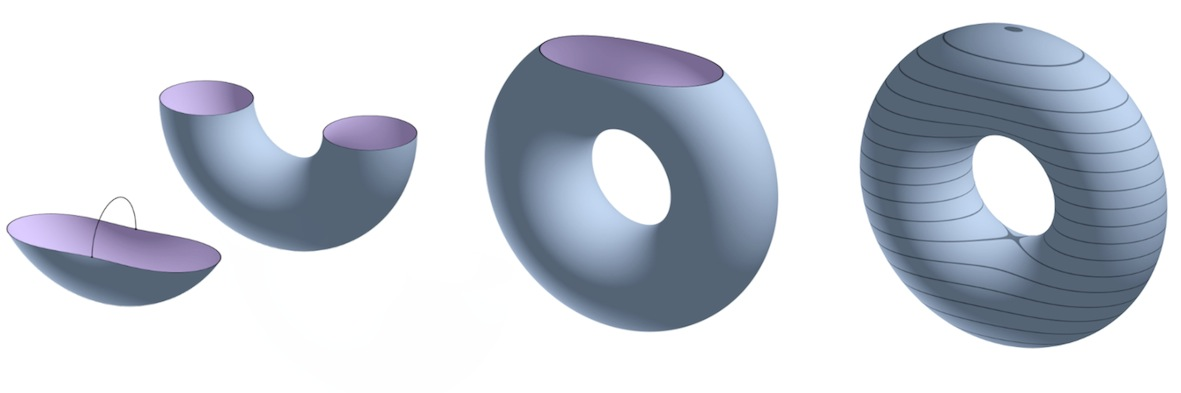
\includegraphics[width=0.90\textwidth]{morse_theory.jpg}
\caption{Morse theory -- starting from the bottom the homotopy type of the torus changes at its critical points from: point or disk, to cylinder, continues to a torus with a removed disk boundary, until it is finally a full torus.}
\label{fig:morse_theory}
\end{figure}\\
The rest of this chapter is split into the following sections: First we will survey previous work in \ref{math_loop_previous_work}, then in section \ref{math_loop_definition} we will proof that there is in fact, always a distinct class of circles that describe the geometric features we are interested in.
Afterwards we define topological persistence in section \ref{math_topological_persistance} and see how it may help us, and finally in \ref{math_loop_computation} we explain how to find the loops computationally.

\subsection{Previous Work}
\label{math_loop_previous_work}

Numerous papers have been published dealing with non-trivial loops on surfaces, as they hold important topological information.
For a good overview, see the references in \citep[][especially section 2]{Ni2004}.
For our thesis, we will focus on preceding work with a explicit context in simplification.
Below are some references with descriptions:
%List \vspace{-2ex}
\begin{itemize}
%\setlength{\itemsep}{0cm}
%\setlength{\parskip}{0cm}
	\item \citep[][]{El-Sana1997} \textit{``Controlled Simplification of Genus \dots''}\\
They identify holes and the concavities by extending the concept of $\alpha$-hulls\footnote{ Generalization for the concept of convex hulls as a set of points associated with disks that represent simple curves \citep[introduced by][]{Edelsbrunner1983}.} to polygonal meshes under the $\mathrm{L}_{\infty}$ distance metric and then triangulate parts of the surface that are not accessible for a ball of a defined radius.
	\item \citep[][]{Guskov2001} \textit{``Topological Noise Removal''}\\
Propose a surface growing strategy to find features and remove unnecessary non-trivial topology. They use a local wave front traversal to discover and identify small tunnels. Then they find and select non-separating cuts to sever and seal the mesh, thus reducing the genus.
	\item \citep[][]{Nooruddin2003} \textit{``Simplification \dots Using Volumetric Techniques''}\\
Describe a method for converting polygonal models to a volumetric representation. The topology altering part is based on 3D morphological operators that work in the volume domain.
	\item \citep[][]{Wood2004} \textit{``Removing Excess Topology From Isosurfaces''}\\
They find handles by incrementally constructing and analyzing Reeb graphs\footnote{ Named after \textit{Georges Reeb}, these graphs of a function describe the connectivity of its level sets -- for figure \ref{fig:morse_theory} the graph would be formed by two edges connected bottom and top of a circle.}. Handles are removed robustly by modifying the volume in a disk-filling procedure.
	\item \citep[][]{Dey2007} \textit{``On Computing Handle and Tunnel Loops''}\\
Using the concept of topological persistence, they filter a manifold to get a set of simplices that are linked to edges that form handle and tunnel loops.
The main advantage of this approach is, that unlike others, it can provide a mathematical guarantee to find relevant topological features without introducing artifacts.\\
Hence we follow this idea\footnote{ The work of \textit{Tamal K. Dey} was first brought to our attention in a discussion with \textit{Tamy Boubekeur}.} and built upon their work as described in section \ref{math_loop_computation}.
\end{itemize}

\subsection{Definition \& Existence of Handle and Tunnel Loops}
\label{math_loop_definition}

One goal for this thesis is, not only to preserve, but to control topology.
This entails mathematically having to define even very intuitive concepts like handles and tunnels.
Formally this was first done in reference to mesh simplification by \citep[][]{Dey2007}.
%Figure
\begin{figure}[htb]
\centering
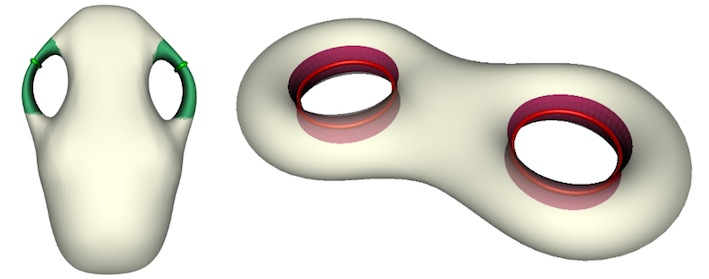
\includegraphics[width=0.66\textwidth]{loop_handle.jpg}
\caption{Handles (green) and tunnels (red) with their defining loops \citep[][]{Dey2012}.}
\label{fig:loop_handle}
\end{figure}\\
A loop defines a handle if it spans a disk in the bounded space bordered by the surface.
If one cuts the surface along such a loop and fills the boundaries with two disks, the handle is eliminated.
Similarly, a tunnel loop spans a disk in the unbounded space bordered by the surface, see figure \ref{fig:loop_handle}.\\
Formalizing this description, let $\mathcal{M}$ be a compact, orientable surface without boundary, i.e. closed and embeddable.
If $\mathcal{M}$ reside inside a $3$-sphere\footnote{ The reason why $\mathcal{M}$ gets embedded in $\mathcal{S}^{3}$, which is a compactification of $\mathbb{R}^{3}$, is to make notations of proofs easier since the space in consideration is finite.}, it separates $\mathcal{S}^{3}$ into two parts $\{(\mathcal{S}^{3} \backslash \mathcal{M})\}$, namely the inside $\mathbb{I}$ and the outside $\mathbb{O}$.
Note that $\mathcal{M}$ is part of both $\mathbb{I}$ and $\mathbb{O}$, analogous to two adjacent triangles that share an edge.
%List \vspace{-2ex}
\begin{itemize}
\setlength{\itemsep}{0cm}
\setlength{\parskip}{0cm}
	\item A tunnel loop is a loop of which the homology class is trivial in $\mathrm{H}^{1}(\mathbb{O})$ and non-trivial in $\mathrm{H}^{1}(\mathbb{I})$.
	\item Accordingly a handle loop has a trivial homology class in $\mathrm{H}^{1}(\mathbb{I})$ and a non-trivial in $\mathrm{H}^{1}(\mathbb{O})$.
\end{itemize}

In other words, handles and tunnels are characterized by the fact that they can be contracted to a point on the inside but are incontractible from the outside and vice versa.
By definition, the set of tunnel loops are disjoint from the set of handle loops, i.e. no handle can be at the same time a tunnel and conversely.
However, not every non-trivial loop on $\mathcal{M}$ is either a handle or a tunnel and both conditions have to be fulfilled, see figure \ref{fig:loop_nontrivial}.

It can be shown shown that for any connected closed surface $\mathcal{M} \subset \mathcal{S}^{3}$ of genus $g$, there exist exactly g handle and tunnel loops: $\{\mathrm{c}^{handle}_{i}, \mathrm{c}^{tunnel}_{i}\}$, with $0 < i \leq g$ forming a basis for $\mathrm{H}(\mathbb{O})$, respectively $\mathrm{H}(\mathbb{I})$.
Furthermore the homology class of circles, that is represented by $[\mathrm{c}^{handle}_{i}]$ and $[\mathrm{c}^{tunnel}_{i}]$ form a basis for $\mathrm{H}^{1}(\mathcal{M})$, which relates them directly to the Betti number $\beta^{1}$, as expected, and will be of great importance in subsection \ref{math_persistence}.\\
The proof involves more algebraic topologic than what was already covered, especially Mayer–Vietoris sequences, therefore we omit the technicalities but instead describe the idea behind it.\\
We saw that $\mathcal{M}$ bisects the space in which it is embedded, $\mathcal{S}^{3} = \mathbb{I} \cup \mathbb{O}$.
Hence it follows that: $\mathrm{H}^{1}(\mathcal{M}) = \mathrm{H}^{1}(\mathbb{I}) \oplus \mathrm{H}^{1}(\mathbb{O})$, with the direct sum of abelian groups.
More importantly it also holds that:
\begin{equation}
rank(\mathrm{H}^{1}(\mathcal{M})) = rank(\mathrm{H}^{1}(\mathbb{I})) + rank(\mathrm{H}^{1}(\mathbb{O})) = 2g
\end{equation}
For symmetry reasons it can be inferred that actually: $rank(\mathrm{H}^{1}(\mathbb{O})) = rank(\mathrm{H}^{1}(\mathbb{I}))$, thus proving that a $2$-manifold of genus g, will always have g tunnel and handle loops.
%Figure
\begin{figure}[htb]
\centering
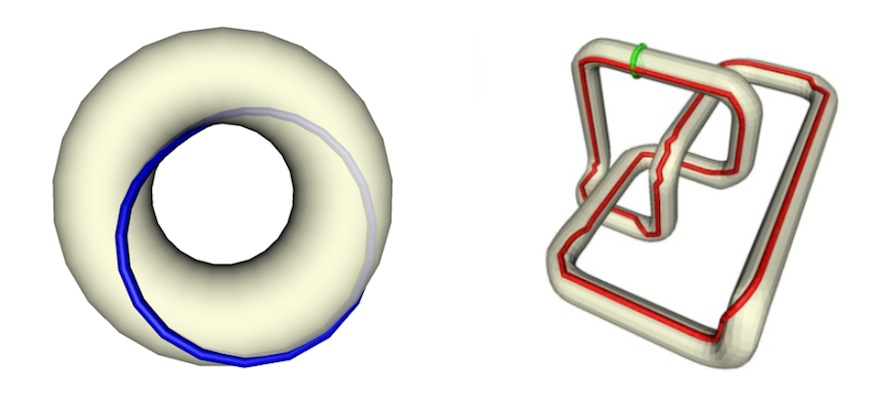
\includegraphics[width=0.66\textwidth]{loop_nontrivial.jpg}
\caption{Left: A non-trivial loop that is neither a handle nor a tunnel, Right: Loops on knotted surface reject the divide in $\mathrm{H}^{1}(\mathbb{I})$ and $\mathrm{H}^{1}(\mathbb{O})$ \citep[][]{Dey2012}.}
\label{fig:loop_nontrivial}
\end{figure}\\
Although this theorem assures the existence of handle and tunnel loops on all connected closed surfaces, they do not bear intuitive meaning on knotted surfaces.
Figure \ref{fig:loop_nontrivial} shows such a surface, which is obtained by thickening a trefoil knot.
Contrary to the natural intuition the red loop is not a tunnel loop.
It is not trivial in $\mathrm{H}^{1}(\mathbb{O})$ yet it can be shown that it generates $\mathrm{H}^{1}(\mathbb{I})$.
This problems can be ameliorated but it introduces unnecessary complexity and consequently we restrict any manifold from here on to be knot free, which is not a problematic restriction in practice.\\

%\newpage
\subsection{Topological Persistence}
\label{math_topological_persistance}

The concept of persistent homology has been introduced, independently by \textit{Robins} \citep[][]{Robins1999} and \textit{Edelsbrunner} \citep[cf.][]{Edelsbrunner2000}.
It provides a mathematical tool, along with a combinatorial algorithm, to capture geometric shapes and is closely related to spectral sequences, mathematical ideas that have been developed 50 years ago\footnote{ See the glossary in \ref{appendix_glossary} and chapter 1.4 of \citep[][]{Zomorodian2005} for more information.}.\\
The main idea behind it, is to study the topological changes of a mesh during an induced growth process and to keep track of how long a topological change lasts, that was induced by a  certain simplex.
This is done by monitoring the homology groups and Betti numbers.\\
In order to measure the longevity of a topological feature, we need two further ingredients, one geometric, assigning a function to a space, the other algebraic, turning the function into measurements.
The measurements make sense, only if the function does, which is studied by substituting an ordering of the simplices for the function\footnote{ This section and its figures are compiled, from the papers: \citep[cf.][]{Delfinado1995}, \citep[cf.][]{Edelsbrunner2000}, \citep[cf.][]{Edelsbrunner2001}, \citep[cf.][]{Zomorodian2008} and \citep[cf.][]{Edelsbrunner2006}. It seems one scholar focused, but not only did \textit{Edelsbrunner} lay the foundations of the field, he is also one of the most highly cited researchers, see: \href{http://researchanalytics.thomsonreuters.com/highlycited/categories/computer_science/}{ISI Highly Cited}. For a complete introduction, a thorough survey of the entire field and the current research, see \citep[][]{Kozlov2008}.}.

\subsubsection{Filtration}
\label{math_filtration}

Let $\mathrm{K}$ be a simplicial complex. A filtration is a nested sequence of subcomplexes and we may think of the filtration as a description of how to construct $\mathrm{K}$ by adding individual parts of it, one after another: $\emptyset = \mathrm{K}_{-1} \subset \mathrm{K}_{0} \subset \mathrm{K}_{1} \subset \dots \subset \mathrm{K}_{n} = \mathrm{K}$\\
More than in the sequence of complexes, we are interested in their topological evolution, expressed by the corresponding sequence of homology groups.
This is possible, since for every $\mathrm{K}_{n-1} \subset \mathrm{K}_{n}$ with $n \geq 1$, the inclusion map induces a homomorphism between the homology groups: $f : \mathrm{H}(\mathrm{K}_{n-1}) \rightarrow \mathrm{H}(\mathrm{K}_{n})$.
Hence, the nested sequence of complexes corresponds to sequences of connected homology groups:
\begin{equation} \label{eq:filtration_persistence}
	0 = \mathrm{H}(\mathrm{K}_{0}) \rightarrow \mathrm{H}(\mathrm{K}_{1}) \rightarrow \dots \rightarrow \mathrm{H}(\mathrm{K}_{n}) = \mathrm{H}^{p}(\mathrm{K})
\end{equation}
Where $p$ represents the homomorphism for each dimension, corresponding to the type of $n$-simplices.
As a consequence the filtration defines a partial ordering on the simplices with: $\sigma_{early} \in (\mathrm{K}_{n-1}-\mathrm{K}_{n})$ preceding $\sigma_{late} \in (\mathrm{K}_{n}-\mathrm{K}_{n+1})$.\\
This total ordering can be extended by deciding on the ordering of the simplices within each $\mathrm{K}_{n-1}-\mathrm{K}_{n}$.
For simplicity one can assume that this ordering consists in the addition of a single simplex at a time.
In other words, the simplices of $\mathrm{K}$ are ordered as $\sigma_{0}, \sigma_{1}, \dots$ such that $\mathrm{K}_{i} = \{\sigma_{0}, \sigma_{1}, \dots, \sigma_{i}\}$, for each $i \leq n$, avoiding ties that result from the otherwise simultaneous creation of simplices, e.g. when a new edge creates a triangle.\\
For example, a $2$-manifold filtration is executed by first adding all the $0$-simplices (vertices) to the set, then including the $1$-simplices (edges) and finally the $2$-simplices (triangle planes), see also figure \ref{fig:filtration_sequence} and the description in the next subsection.

\subsubsection{Incremental Betti Numbers}
\label{math_incremental_betti}

The ordering of simplices in a filtration permits a simple algorithm for computing Betti numbers.
Suppose the sequence of $K_{i} = \{ \sigma_{j} \,|\, 0 \leq j \leq i \}$, for $i \leq n$.
The initial Betti numbers for the set of the empty simplicial complex is obviously $\beta^{0} = \beta^{1} = \beta^{2} = 0$, and the algorithm then works as follows:
%Algorithm
\begin{table}[htb] \bigskip \centering
\setlength{\tabcolsep}{5pt}
\renewcommand{\arraystretch}{1.10}
\fbox{
	\begin{minipage}{10cm}
	\begin{tabular}{l | l} 
			&	\textsc{Betti-numbers ()} \\[1ex]
		\tiny{1}	&	\hspace{0.2cm}	\textsf{for $i=0$ to $n-1$ do} \\
		\tiny{2}	&	\hspace{1.0cm}	\textsf{$k = dim(\sigma_{i}) - 1$} \\
		\tiny{3}	&	\hspace{1.0cm}	\textsf{if $\sigma_{i}$ belongs to a (k+1)-cycle in $\mathrm{K}_{i}$} \\
		\tiny{4}	&	\hspace{1.5cm}	\textsf{then $\beta^{k+1} = \beta^{k+1}+1$} \\
		\tiny{5}	&	\hspace{1.5cm}	\textsf{else $\, \beta^{k} = \beta^{k}-1$} \\
		\tiny{6}	&	\hspace{1.0cm}	\textsf{endif} \\
		\tiny{7}	&	\hspace{0.2cm}	\textsf{endfor} \\
		\tiny{8}	&	\hspace{0.2cm}	\textsf{return $(\beta^{0}, \beta^{1}, \beta^{2})$} \\[1ex] 
	\end{tabular} \end{minipage}
}
	\medskip
	\caption{Algorithm -- Betti numbers of simplicial complexes.}
	\label{algo:betti_numbers}
\end{table}\\
The only question remaining is, how to decide whether a simplex $\sigma_{i}$ belongs to a cycle in $\mathrm{K}_{i}$, or not? 
For vertices $dim(\sigma_{i}) = 0$ it is defined, since every connected vertex belongs automatically to a $0$-cycle\footnote{ We imply that there are no ``free floating'' unconnected vertices allowed in the set $\mathrm{K}$.}.
To decide this for edges, we have to maintain a representation of the connected components, since an edge belongs to a $1$-cycle if and only if its two endpoints belong to the same component, i.e. if it closes a triangle.
Triangles $dim(\sigma_{i})=2$ are treated similarly, checking correspondence with $2$-cycles.\\
This definition sounds rather abstract, but can be easily made clear by showing a filtration.
We call a simplex positive $\Prefix^{+}{\sigma}$, if it belongs to a cycle and negative $\Prefix^{-}{\sigma}$, if it doesn't.
In figure \ref{fig:filtration_sequence}, a filtration is depicted that builds a tetrahedron with a flag.
Each step, shown by the number in the lower left box, adds one simplex to the set $\mathrm{K}_{i}$ with $0 \leq i \leq 17$.
%Figure
\begin{figure}[htb]
\centering
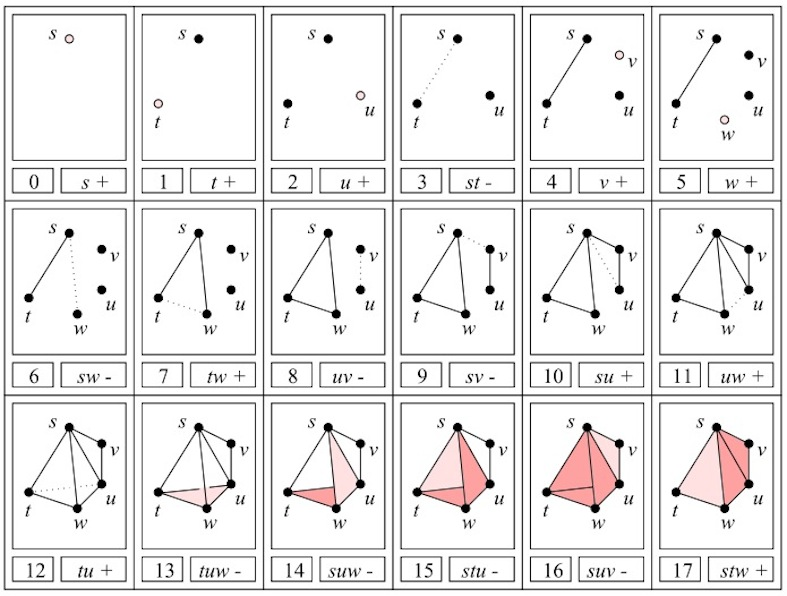
\includegraphics[width=0.75\textwidth]{filtration_sequence.jpg}
\caption{Example of a filtration sequence, building a tetrahedron with flag triangle.}
\label{fig:filtration_sequence}
\end{figure} \vspace{-2ex}
\begin{itemize}
  \setlength{\itemsep}{0cm}%
  \setlength{\parskip}{0cm}%
	\item Vertices $\{s, t, u, v, w\}$ increment $\beta^{0}$ -- steps: $0, 1, 2, 4, 5 ~\longrightarrow~ \beta^{0} = +5$
	\item Edges $\{st, sw, uv, sv\}$ decrement $\beta^{0}$ -- steps: $3, 6, 8, 9 ~\longrightarrow ~\beta^{0} = +5-4$
	\item Edges $\{tw, su, uw, tu\}$ increment $\beta^{1}$ -- steps: $7, 10, 11, 12 ~\longrightarrow ~\beta^{1} = +4$
	\item Faces $\{tuw, suw, stu, suv\}$ decrement $\beta^{1}$ -- steps: $13, 14, 15, 16 ~\longrightarrow ~\beta^{1} = +4-4$
	\item Face $\{stw\}$ increments $\beta^{2}$ -- step: $17 ~\longrightarrow ~\beta^{2} = +1$
\end{itemize}
We can now summarize the incremental steps and get: $\beta^{0} = 1, \,\beta^{1} = 0, \,\beta^{2} = 1$ meaning that there is one component with no non-trivial loops, encapsulating one void.
Also, since $\chi(\mathrm{K}) = \sum_{i} (-1)^{i}\beta^{i} = +1 -0 +1 = 2$, we verify the result with what we already know about compact and orientable $2$-manifolds that have no holes, namely their Euler characteristic of $\chi = 2$.
The correctness of the incremental algorithm implies:
\begin{equation} \label{eq:incremental_betti}
	\beta^{i} = |\Prefix^{+}{\sigma^{i}}|-|\Prefix^{-}{\sigma^{i+1}}| \text{ for } i \geq 0
\end{equation}
In other words, the $i^{th}$-Betti number $\beta^{i}$ is the number of $i$-simplices that create $i$-cycles minus the number of ($i$+1)-simplices that destroy $i$-cycles by creating $i$-boundaries.

\subsubsection{Persistent Homology}
\label{math_persistence}

The idea of persistent homology can be described as a measure that ranks attributes by their lifetime in a filtration.
To asses the persistence for a topological feature in the face of growth, positive and negative simplices are being paired\footnote{ We haven't explicitly discussed the relation between positive and negative simplices and omit a proof, but since every Betti number $\beta^{i} \in \mathbb{N}$, it must follow that for every negative simplex $dim$(i+1) exists a positive simplex $dim(i)$ that it pairs: $|\Prefix^{+}{\sigma^{i}}| \geq |\Prefix^{-}{\sigma^{i+1}}|$. Note that while the pairing depends on the filtration, the number of paired tuples and unpaired positive simplices does not. For a discussion of tracking generating cycles if the simplicial complex or the filtration changes, see \citep[][]{Busaryev2010}.}\label{fn:simplex_relation}.
Although this is only the tip of the iceberg of the theory, for our purposes, the concept of pairing is the only aspect we are interested in\footnote{ Not only can persistent homology be used as an invariant that captures the homological history of an arbitrary space, it also has applications in topological approaches for separating signals from noise and has been utilized in various fields. For example to measure structural changes in membrane fusion, which describe key stages in cellular processes such as virus infections \citep[cf.][]{Kasson2007}.}.\\
Figure \ref{eq:filtration_persistence} visualizes two ways of illustrating the pairing of simplices from the filtration process in figure \ref{fig:filtration_sequence}.
Either with half open intervals $[\Prefix^{+}{\sigma_{i}}, \Prefix^{-}{\sigma_{j}})$, or by the two dimensional representation that spans triangles.
The light triangles represent $0$-cycles, the dark ones $1$-cycles and the area indicates the perseverance of a simplex:
%Figure
\begin{figure}[htb]
\centering
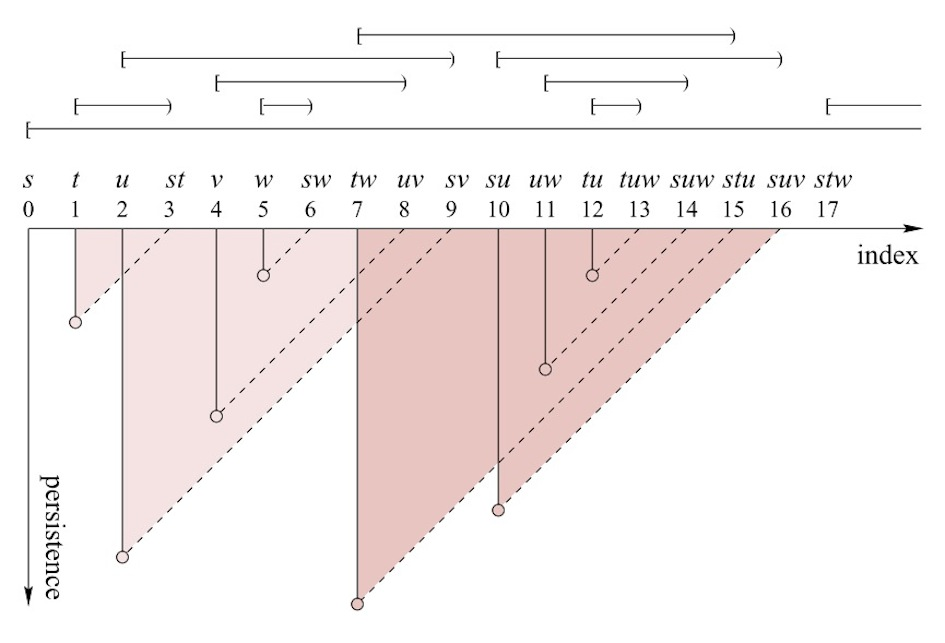
\includegraphics[width=0.60\textwidth]{persistent_homology.jpg}
\caption[Persistence of the simplices]{Persistence of the simplices.}
\label{fig:persistent_homology}
\end{figure}\\
One might note that the vertex $\{s\}$ and the face $\{stw\}$ are unbounded and not drawn.
This is a consequence of equation \eqref{eq:incremental_betti} and means that for every increment of $\beta^{i}$ an unpaired  positive simplex $\Prefix^{+}{\sigma^{i}}$ gets associated that belongs to the homology group of the generating set, i.e the basis.
In other words, each simple connected manifold $\beta^{0} = 1$, has a representative vertex $\sigma^{0}$ and for every non-bounding $1$-cycle, represented by $\beta^{1}$, there is an edge that belongs to a collation of non-contractible closed curves, an so forth.\\
Formally the reasoning behind this observation combines and concludes the work of the entire chapter and will finally explain why we are interested in all of this, as we initially set out to identify certain geometrical features, specifically handles and tunnels.
Combining the relations of $\beta$ as introduced in equations \ref{eq:euler_poincare}, \ref{eq:homology_betti} and \ref{eq:incremental_betti}, we get:
%Equation
\begin{equation} \label{mother_equation}
	\underbrace{ \chi = \sum (-1)^{n} \, \beta^{n}}_{Euler-Poincaré}
	\hspace{3ex} \longrightarrow \hspace{1ex}
	\underbrace{ \beta^{n}}_{n-Betti} =
	\underbrace{ rank ~{Z}^{n} - rank ~\mathrm{B}^{n}}_{Homology~groups} =
	\underbrace{ |\Prefix^{+}{\sigma^{n}}|-|\Prefix^{-}{\sigma^{n+1}}|}_{Filtration}
\end{equation}\\
\underline{Euler-Poincaré:}
Without a question the genus, respectively the Euler characteristic is the most prominent topological invariant.
As intuitive as it might be, it is also very limited in its explanatory reach.
For instance, just judging by $\chi$, there is no way to discriminate whether a tunnel of a manifold was closed or new objects added to the set. 
Therefore we refine the concept with the help of Betti numbers.\\
 \underline{$n$-Betti:} In this way, controlling the topology translates to tinkering with Betti numbers.
Since we are generally not interested in modeling but simplifying the surfaces, we focus on decreasing Betti numbers.
For the most part we deal with just one simple connected manifold, hence $\beta^{0} = 1$ is unchangeable and of minor importance.
Neither is the amount of enclosed voids, denoted by $\beta^{2}$, as it pertains to the characteristics of the interior.
Surfaces do not have $\beta^{i} \neq 0$ with $i \geq 3$, so by exclusion the only really importance falls onto $\beta^{1}$, describing the amount of disjoint non-contractible circles.\\
 \underline{Homology groups:} The integer that represents $\beta^{1}$ actually represents an entire group of circles that belong to the same homologic group.
Consequently we have to expand the concept as we did with the genus that was refined into the Euler-Poincaré formula.
This is achieved by examining the relation of chains in general and specifically the subgroup of chains that bind cycles\footnote{ Hinted by the fact that we introduced $ranks, kernels$ and $images$, it is not surprising that persistence can also be nicely explained in terms of matrix operations, which is a field of study in itself \citep[see chapters IV-3 and VI-1 in][]{Edelsbrunner2006}.}, also see figure \ref{fig:chain_complex}.\\
\underline{Filtration:} The final step is finding one representative circle from the entire homologic group.
To narrow down the selection, we use filtration, as it identifies edges that are boundaries for the circles in question.
That is to say, that after all the mathematical machinery that was put into motion we have firmly proven that for every tunnel or handle of a manifold we can compute an edge that is part of the defining loop.
What is left now, is an exact description of these loops and the algorithm, given in section \ref{math_loop_definition} and \ref{math_loop_computation}.

\subsection{Computing Geometry-aware Loops}
\label{math_loop_computation}

At the end of the last subsection we concluded that if we pair simplices during a filtration, we acquire a set $\mathbb{U} = \{ \Prefix^{+}{\sigma}\}$ of unpaired positive simplices.
We are interested in the subset of simplices $\Prefix^{+}{\sigma^{p}}$ of dimension $p = 1$: $\,\mathbb{U}^{1} \subset \mathbb{U}$  with $|\mathbb{U}^{1}| = 2g$, as this subset consists of edges that represent the tunnel and handle loops of the surface.\\
We now describe the principal steps\footnote{ The following algorithms were first described and proven in \citep[][]{Dey2007} and later refined and sped-up in \citep[][]{Dey2008, Dey2009}. Basically we follow the ideas for pairing simplices, but deviate in the latter stages when optimizing the found loops.} necessary to generate this set and afterwards discuss the two building algorithms in more detailed in subsection \ref{math_algorithm_pairing} and \ref{math_algorithm_looprefinement}.\\
%List
\vspace*{-1.0cm}
\begin{enumerate}
\setlength{\itemsep}{0cm}
\setlength{\parskip}{0.15cm}
\item The input is a simplicial complex $\mathrm{K}_{S}$ that constitutes a closed, orientable surface $\mathcal{M}$. By using a Delaunay meshing algorithm\footnote{ We used the freely available implementation named \href{http://tetgen.berlios.de/}{TetGen} for that purpose \citep[cf.][]{Si2010}.}, one obtains the tessellated convex hull of $\mathcal{M}$, i.e. the simplicial representations for the inside $\mathrm{K}_{\mathbb{I}}$ and the outside $\mathrm{K}_{\mathbb{O}}$, that together form $\mathrm{K} = \mathrm{K}_{S} \cup \mathrm{K}_{\mathbb{I}} \cup \mathrm{K}_{\mathbb{O}}$. Although we are only interested in the circles on $\mathrm{K}_{S}$, we need triangles for the inside and the outside in order to add them to our filtration and find not only unpaired edges but also their corresponding loops.
\item The simplices of the surface $\mathrm{K}_{S}$ are added to filtration in an arbitrary order. Paring each of them with the algorithm described in \ref{math_algorithm_pairing}, gives $2g$ unpaired edges $\mathbb{U}^{1}$.
\item The simplices of $\mathrm{K}_{\mathbb{I}}$ are added to the filtration. Which pairs half of the edges in $\mathbb{U}^{1}$ with negative triangles $\Prefix^{-}{\sigma_{i}^{2}}$ and associates an explicit circle to each edge, i.e. the one that got killed by $\Prefix^{-}{\sigma_{i}^{2}}$, which by definition is a handle loop. The filtration with $\mathrm{K}_{\mathbb{I}}$ can be stopped as soon as $g$ edges of $\mathbb{U}^{1}$ are paired with their circles $\{c^{1}_{handle~i}\}^{g}_{i=1}$, see figure \ref{fig:unpaired-edges_paired-loops} illustrating the steps 2-4.
\item Lastly the simplices of $\mathrm{K}_{\mathbb{O}}$ are included into the filtration. The remaining positive edges in $\mathbb{U}^{1}$ get paired as before, thereby obtaining $g$ more circles that are by definition tunnel loops $\{c^{1}_{tunnel~i}\}^{g}_{i=1}$. Note that loops that get killed by negative triangles in $\mathrm{K}_{\mathbb{I}}$ or $\mathrm{K}_{\mathbb{O}}$ have all their edges lying on $\mathrm{K}_{S}$ because the simplices of the inside and outside only get added after all simplices of $\mathrm{K}_{S}$ are in the filtration.
\item The computed loops are undoubtedly correct as far as homology is concerned, but as can be seen in figure \ref{fig:unpaired-edges_paired-loops}, they are not necessarily appealing in a geometrical sense. For that reason we refine the loops as described in \ref{math_algorithm_looprefinement}.
\end{enumerate}
%Figure
\begin{figure}[htb]
\centering
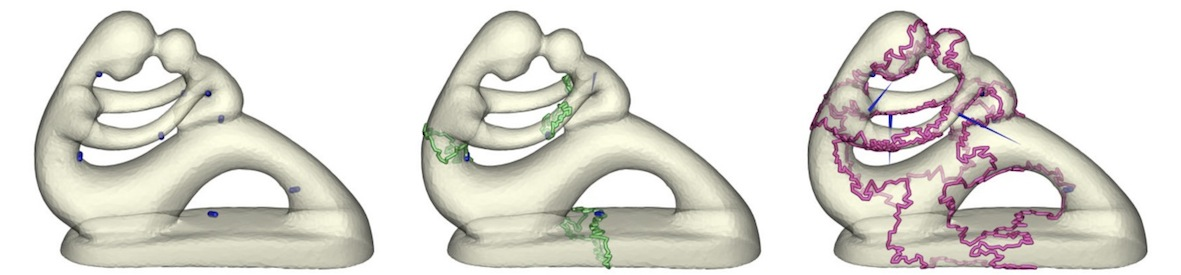
\includegraphics[width=1.0\textwidth]{unpaired-edges_paired-loops.jpg}
\caption{Left to right: Unpaired edges,handle loops and tunnel loops \citep[][]{Dey2012}.}
\label{fig:unpaired-edges_paired-loops}
\bigskip
\end{figure}

\subsubsection{Pairing Algorithm}
\label{math_algorithm_pairing}

Pairing is the essential concept of persistent homology, as it determines the lifetime, i.e. persistence of $n$-cycles.
In order to pair the simplices, we have to determine whether they are negative or positive.
Recall that a simplex $\sigma^{n}$ of dimension $n$, is positive $\Prefix^{+}{\sigma^{n}}$, if it creates a non-bounding $n$-cycle and that it is negative $\Prefix^{-}{\sigma^{p}}$, if it kills an existing ($n$-1)-cycle.
In other words, every new edge $\sigma^{1}$ kills a $0$-cycle, unless it closes a chain $\mathrm{c} = \{ \sigma^{1}_{0}, \sigma^{1}_{1}, \dots , \sigma^{1}_{i} \}$ so that $\partial (\mathrm{c} + \sigma^{1}) = \emptyset$.
In the exemplary case shown in figure \ref{fig:filtration_sequence}, it is not hard to figure the sign out $\Prefix^{\pm}{\sigma}$, but for an arbitrarily large simplicial complex $K$, we need a more elaborate approach using the notion of temporality -- introduced as a consequence of equation \eqref{eq:filtration_persistence}, we defined that for every step in a filtration, exactly one additional simplex gets added with that the latest addition being the youngest simplex of the complex.
Generally speaking $\sigma_{j} = \mathrm{K}_{j} - \mathrm{K}_{j-1}$ is younger than $\sigma_{i} = \mathrm{K}_{i} - \mathrm{K}_{i-1}$, if it appears later in the filtration, i.e. $\mathrm{K}_{j} \supset \mathrm{K}_{i}$.

We analyze parts of the filtration from example \ref{fig:filtration_sequence} to see how the algorithm works before we give a formal description in \ref{algo:simplex_pairing}.\\
In the stage $\mathrm{K}_{3}$ of the process the first edge gets added, before that only the vertices $\sigma^{0}_{0}$ up to $\sigma^{0}_{2}$ populate the simplicial complex. 
All vertices are trivially positive, as there are no ($p$-1)-cycles that could be closed.
This can be shown formally: $\partial \sigma^{0} = \partial \{v\} = \emptyset \,\rightarrow \,\Prefix^{+}{\sigma^{0}}$, since the boundary operator, applied to any vertex, results in the empty set.
Now to pair the new edge $\sigma^{1}_{3} = \{s,t\}$, we check its boundary: $c = \partial \sigma^{1}_{3} = \partial \{s,t\} = (s+t)$.
No circle was closed, which would have left the the boundary empty, thus must be negative and we can pair the simplex with the youngest candidate.
By convention we always assign the youngest unpaired positive simplex to the pair, in this case this is vertex $t$ as it is younger than $s$: $\sigma^{0}_{1} > \sigma^{0}_{0}$ and we get the pairing: $\langle t, st \rangle = \langle \Prefix^{+}{\sigma^{0}_{1}}, \Prefix^{-}{\sigma^{1}_{3}} \rangle$, which is visualized as the first triangle in figure \ref{fig:persistent_homology}.
Now we look at step $\mathrm{K}_{7}$ that introduces the edge $\sigma^{1}_{7}$, that closes a triangle.
More precisely: $c = \partial \sigma^{1}_{7} = \partial \{t, w\} = (t + w)$, but since $t$ and $w$ are already paired, we have to add their pairs respectively their boundaries: $(t + w) = (t + \{s,t\} + w + \{s,w\}) \rightarrow (t + \partial \{s,t\} + w + \partial \{s,w\}) = (t + s + t + w + s + w) = (2s + 2t +2w)$, note that we defined the addition modulo 2: $(2s + 2t +2w) = \emptyset \rightarrow \Prefix^{+}{\sigma^{1}_{7}}$, meaning that the edge is positive.
Generalizing this for the entire simplicial complex, gives us the pairing algorithm:
%Algorithm
\begin{table}[htb] \medskip \centering
\setlength{\tabcolsep}{5pt}
\renewcommand{\arraystretch}{1.2}
\fbox{
	\begin{minipage}{10cm}
	\begin{tabular}{r | l} 
			&	\textsc{Pairing ($\sigma$)} \\[1ex]
		\tiny{1}	&	\hspace{0.2cm}	\textsf{$\mathrm{c} = \partial \sigma^{p} = \{ \sigma_{i}^{p-1}, \dots , \sigma_{j}^{p-1}  \}$} \\
		\tiny{2}	&	\hspace{0.2cm}	\textsf{let $\sigma_{last}$ be the youngest ($p$-1)-simplex in $\mathrm{c}$} \\
		\tiny{3}	&	\hspace{0.2cm}	\textsf{while $\sigma_{last}$ is paired and $\mathrm{c} \neq \emptyset$ do} \\
		\tiny{4}	&	\hspace{1.0cm}	\textsf{let $c_{kill}$ be the cycle which was killed by $\sigma_{last}$} \\
		\tiny{5}	&	\hspace{1.0cm}	\textsf{$c = c + c_{kill}$} \\
		\tiny{6}	&	\hspace{1.0cm}	\textsf{update $\sigma_{last}$ to the youngest ($p$-1)-simplex in $c$} \\
		\tiny{7}	&	\hspace{0.2cm}	\textsf{end while} \\
		\tiny{8}	&	\hspace{0.2cm}	\textsf{if $c \neq \emptyset$ then} \\
		\tiny{9}	&	\hspace{1.0cm}	\textsf{the simplex is negative $\Prefix^{-}{\sigma}$, killing $c$} \\		
		\tiny{10}	&	\hspace{1.0cm}	\textsf{pair $(\sigma_{last}, \Prefix^{-}{\sigma})$} \\
		\tiny{11}	&	\hspace{1.0cm}	\textsf{associate $c$ as $c_{kill}$ with the simplex $(c_{kill}, \Prefix^{-}{\sigma})$} \\
		\tiny{12}	&	\hspace{0.2cm}	\textsf{else} \\
		\tiny{13}	&	\hspace{1.0cm}	\textsf{the simplex is positive $\Prefix^{+}{\sigma}$} \\
		\tiny{14}	&	\hspace{0.2cm}	\textsf{end if} \\[1ex]
	\end{tabular} \end{minipage}
}
	\medskip
	\caption{Algorithm -- Simplex pairing.}
	\label{algo:simplex_pairing}
\end{table}\\
The algorithms spends most of its time expanding $c = \partial \sigma$ in order to decide whether at the end it is empty or not.
We can speed the process up by introducing another condition for the \textsf{while} loop.
It relies on the observation that, at no time during the expansion of $c$, the youngest simplex in $c$ can be older than the oldest simplex in $\mathbb{U}^{1}$, without it automatically being a positive simplex.
This means that if $\sigma_{last} < \Prefix^{+}{\sigma_{last\,\mathbb{U}}} \,\rightarrow \, \Prefix^{+}{\sigma_{last}}$.
The comparison is easy to do, as we only have to check the indices $j$ and $i$ of the corresponding stage of the filtration: $\sigma_{last} = \mathrm{K}_{j} - \mathrm{K}_{j-1}$ and $\Prefix^{+}{\sigma_{last\,\mathbb{U}}} = \mathrm{K}_{i} - \mathrm{K}_{i-1}$.\\
The observation can be formally proven but it is explicitly clear, considering the fact that after the filtration of $\mathrm{K}_{\mathcal{S}}$, only positive simplices are unpaired and that it is not possible to be left with unpaired negative simplices at that point\footnote{ See the first footnote on page \pageref{fn:simplex_relation} for more explanation.}.

\subsubsection{Refining the Loops}
\label{math_algorithm_looprefinement}

After the entirety of this chapter we are now finally at the point where we actually have the loops representing the topological features we wanted to find, namely handles and tunnels.
To be precise, we have a number of homologous circles that we acquire in the \textsf{while} loop of algorithm \ref{algo:simplex_pairing}.
During the process of finding the paired positive edges for a negative triangle we get a series of them and now have to choose one among them.

The previous work of \citep[][]{Dey2007, Dey2008, Dey2009} has devoted considerable effort to perfect the selection by two methods: 
One is to assign geodesic sizes to the triangles in $\mathrm{K}_{\mathbb{I}}$ and $\mathrm{K}_{\mathbb{O}}$, respectively the projection of their edges onto the surface.
This is done to then order them according to size and introduce them, smallest triangle first to the filtration, thereby ensuring to pair smaller loops first.
The other method drops the idea to connect the handle and tunnel loops to their unpaired positive edges all together.
Instead the shortest circle in the homology class is searched, broadening the search immensely.
%Figure
\begin{figure}[htb]
\centering
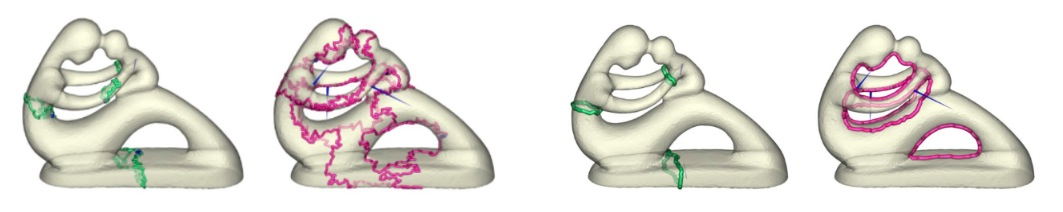
\includegraphics[width=1.0\textwidth]{loop_refinement.jpg}
\caption{Initial results and refined loops on the right \citep[][]{Dey2009}.}
\label{fig:loop_refinement}
\end{figure}\\
These two refinements undoubtedly improve the geometrical appearance greatly, as seen in figure \ref{fig:loop_refinement}.
However we find the prize in computational expenses to be too high.\\
The only costly stage in the entire sequence thus far has been the Delaunay triangulation, which we consider to be a pre-process that can be automated and done in advance.
One advantage of the persistence based algorithm is that it is combinatorial in nature and thereby avoids costly, error-prone numerical computations.
Unlike many previous methods, the algorithm does not require computing any extra data structures such as Reeb graphs, medial axes, or curve skeletons\footnote{ In 2D, the medial axis of a shape is a set of curves defined as the locus of points that have at least two closest points on the boundary of the shape. In 3D, the corresponding object is also called the medial surface because in addition to curves, it can contain surface patches.\\
Likewise a curve skeleton is an abstract 1D geometrical representation of 3D shapes that considers topological features. By segmenting the object it can help spatial understanding, providing a higher level description of the object.}.
We find it of pivotal importance to try and keep the workflow as fast as possible, not changing workflow regime.
As mentioned in section \ref{introduction4}, we firmly believe that interactivity trumps automation and legitimates then necessary user interaction to obtain similar results.\\
Accordingly our solution for refining the computer loops is to substitute the geodesic metric by a simple edge-count.
This is reasonable given the fact that for most triangle surfaces the edge size does not vary much in local neighborhoods.
To further improve the results we give the user the freedom to manually tweak circles be changing parts of the path.
Not only does this ameliorate the quality chasm between the reference implementation and our solution but also lends itself nicely to the simplification step where the user defines which loops to kill by triangulating them, see section \ref{topstoc0} for the details.

This concludes this chapter \ref{math0}, we have talked about basic topology in section \ref{math1}, as well as more advanced concepts like filtration in section \ref{math2} and found a way to leverage the theory to describe and find topological features.
Having described the algorithms involved we now turn to the actual application of the techniques.
We will discuss in the next chapter \ref{topstoc0}, among other principles, how to put them use.
Resulting in a direct and useful workflow to simplify not only fast and robustly, but also with numerous levers that can be tweaked directly by the user -- one being the control over topology.

% smiley command: $\ddot\smile$
